% ============================================================
% SmartQ — Smart Hospital Queue Management System
% Detailed Academic Report (LaTeX for Overleaf)
% ============================================================
\documentclass[12pt,a4paper]{article}

% ─── Packages ───────────────────────────────────────────────
\usepackage[utf8]{inputenc}
\usepackage[T1]{fontenc}
\usepackage{lmodern}
\usepackage[margin=1in]{geometry}
\usepackage{graphicx}
\usepackage{booktabs}
\usepackage{longtable}
\usepackage{array}
\usepackage{tabularx}
\usepackage{multirow}
\usepackage{enumitem}
\usepackage{amsmath}
\usepackage{hyperref}
\usepackage{xcolor}
\usepackage{listings}
\usepackage{tikz}
\usepackage{float}
\usepackage{caption}
\usepackage{subcaption}
\usepackage{fancyhdr}
\usepackage{titlesec}
\usepackage{setspace}
\usepackage[ruled,vlined,linesnumbered]{algorithm2e}
\usepackage{tocloft}

\usetikzlibrary{shapes.geometric, arrows.meta, positioning, fit, backgrounds, calc}

% ─── Hyperref Setup ─────────────────────────────────────────
\hypersetup{
    colorlinks=true,
    linkcolor=blue!70!black,
    citecolor=blue!70!black,
    urlcolor=blue!70!black,
    bookmarksnumbered=true,
    pdfauthor={},
    pdftitle={SmartQ — Smart Hospital Queue Management System},
    pdfsubject={MADLAB Project Report},
}

% ─── Code Listing Style ─────────────────────────────────────
\definecolor{codebg}{RGB}{248,248,248}
\definecolor{codegreen}{RGB}{0,128,0}
\definecolor{codegray}{RGB}{128,128,128}
\definecolor{codeblue}{RGB}{0,0,180}
\definecolor{codepurple}{RGB}{128,0,128}

\lstdefinestyle{mystyle}{
    backgroundcolor=\color{codebg},
    basicstyle=\ttfamily\footnotesize,
    breakatwhitespace=false,
    breaklines=true,
    captionpos=b,
    commentstyle=\color{codegreen},
    keywordstyle=\color{codeblue}\bfseries,
    numberstyle=\tiny\color{codegray},
    stringstyle=\color{codepurple},
    showstringspaces=false,
    numbers=left,
    numbersep=8pt,
    frame=single,
    rulecolor=\color{black!30},
    tabsize=2,
    xleftmargin=15pt,
    framexleftmargin=15pt,
}
\lstset{style=mystyle}

% ─── Pseudocode listing style ───────────────────────────────
\lstdefinestyle{pseudo}{
    backgroundcolor=\color{codebg},
    basicstyle=\ttfamily\footnotesize,
    breaklines=true,
    frame=single,
    rulecolor=\color{black!30},
    xleftmargin=15pt,
    framexleftmargin=15pt,
    numbers=none,
    showstringspaces=false,
    mathescape=true,
    morekeywords={FUNCTION, IF, THEN, RETURN, ELSE, FOR, WHILE, END, SET, PUSH, REMOVE, UPDATE, FIND, ORDER, BY, ASC, AND, OR, WHERE, SAVE, REJECT, MAX, ROUND, SUM, LENGTH, INDEX},
    keywordstyle=\color{codeblue}\bfseries,
}

% ─── Section Formatting ─────────────────────────────────────
\titleformat{\section}{\large\bfseries\sffamily}{\thesection.}{0.5em}{}
\titleformat{\subsection}{\normalsize\bfseries\sffamily}{\thesubsection}{0.5em}{}
\titleformat{\subsubsection}{\normalsize\itshape\sffamily}{\thesubsubsection}{0.5em}{}

% ─── Header / Footer ────────────────────────────────────────
\pagestyle{fancy}
\fancyhf{}
\fancyhead[L]{\small\textit{SmartQ — Smart Hospital Queue Management System}}
\fancyhead[R]{\small\textit{MADLAB Project Report}}
\fancyfoot[C]{\thepage}
\renewcommand{\headrulewidth}{0.4pt}
\renewcommand{\footrulewidth}{0pt}

% ─── Spacing ─────────────────────────────────────────────────
\setstretch{1.25}

% ─── Custom Commands ─────────────────────────────────────────
\newcommand{\cmark}{\textcolor{green!60!black}{\checkmark}}
\newcommand{\xmark}{\textcolor{red!70!black}{$\times$}}
\newcommand{\dash}{---}

% ============================================================
\begin{document}

% ─── Title Page ──────────────────────────────────────────────
\begin{titlepage}
    \centering
    \vspace*{2cm}
    
    {\Huge\bfseries\sffamily SmartQ}\\[0.5cm]
    {\LARGE\sffamily Smart Hospital Queue Management System}\\[2cm]
    
    {\Large\textbf{Project Progress Report}}\\[0.5cm]
    {\large MADLAB Project — Semester 6}\\[3cm]
    
    \rule{0.6\textwidth}{0.4pt}\\[1cm]
    
    {\Large\textbf{Team Members}}\\[0.5cm]
    {\large
    \begin{tabular}{l@{\hspace{1.5cm}}r}
        Utkarsh Jha & 230953422 \\[0.3cm]
        Mihir Sahay & 230953498 \\[0.3cm]
        Rishi Khandelwal & 230953494 \\[0.3cm]
        Omkar Nayak & 230953502 \\
    \end{tabular}
    }\\[1.5cm]
    
    {\large
    \begin{tabular}{rl}
        \textbf{Subject:} & Mobile Application Development Laboratory \\[0.3cm]
        \textbf{Academic Year:} & 2025--2026 \\
    \end{tabular}
    }
    
    \vfill
    
    {\large\today}
\end{titlepage}

% ─── Table of Contents ──────────────────────────────────────
\newpage
\tableofcontents
\newpage

% ============================================================
% ABSTRACT
% ============================================================
\section*{Abstract}
\addcontentsline{toc}{section}{Abstract}

The outpatient department (OPD) of any hospital is typically the first point of contact between patients and the healthcare system, and it is here that the problems of long waiting times, overcrowded lobbies, and inefficient patient flow are most acutely felt. Despite rapid advances in healthcare technology, a majority of hospitals in India and across developing nations continue to rely on manual, paper-based token systems that offer patients no visibility into expected wait times, no mechanism to defer or adjust their position in the queue, and no automated prioritization for vulnerable groups such as elderly patients. This project, titled \textbf{SmartQ}, addresses these shortcomings by presenting the design, development, and implementation of a full-stack, mobile-augmented smart queue management system specifically tailored for hospital outpatient departments.

SmartQ is composed of two primary components: a \textbf{native Android application} (built in Java using Material Design components) that serves as the patient, doctor, and administrator interface, and a \textbf{Node.js/Express.js RESTful backend API} connected to a \textbf{MongoDB Atlas} cloud database. The system introduces a digital token mechanism where patients can remotely join a specific doctor's queue from their smartphone, receive a sequentially numbered token, and track their live queue position along with a dynamically computed estimated time of arrival (ETA). The ETA is calculated using a moving average algorithm that considers the last ten consultation durations for each doctor, thereby adapting to real-world consultation pace rather than relying on static assumptions.

A key innovation of SmartQ is its \textbf{age-based priority triage algorithm}, which automatically assigns a higher priority score to patients aged 60 and above, and dynamically reorders the queue to position these high-priority patients ahead of normal-priority patients while preserving the ordering among patients of equal priority. The system also features a \textbf{snooze mechanism} that allows patients to defer their turn by a configurable number of positions (with a maximum of two snoozes per visit), a \textbf{manual check-in system} (with planned geofence-based automatic check-in using Google Play Services Location APIs), and a comprehensive \textbf{admin dashboard} that enables hospital staff to call the next patient, mark no-shows with automatic queue compaction, pause and resume queues, and view real-time analytics including average consultation times and patient counts.

The application employs JWT (JSON Web Token)-based stateless authentication with bcrypt password hashing, role-based access control across three user roles (patient, doctor, admin), and persistent session management via Android SharedPreferences. The system architecture follows a client-server model with Retrofit and OkHttp handling the HTTP communication layer, including automatic token attachment via interceptors and graceful session expiry handling on 401 responses.

\vspace{0.5em}
\noindent\textbf{Keywords:} Queue Management System, Hospital OPD, Android Application, Priority Scheduling, REST API, MongoDB, JWT Authentication, Patient Flow Optimization, Mobile Health (mHealth), Real-time ETA.

\newpage

% ============================================================
% 1. INTRODUCTION
% ============================================================
\section{Introduction}

Healthcare delivery in India presents a unique set of challenges that are fundamentally different from those faced in developed nations. Government hospitals and large public healthcare institutions routinely serve thousands of outpatients daily, and the physical infrastructure is often insufficient to accommodate the volume of patients seeking consultation. The outpatient department, which functions as the gateway to specialized care, is particularly affected by this mismatch between demand and capacity. Patients arriving at hospitals frequently encounter disorganized queues, with no systematic way to determine how long they will have to wait or how many patients are ahead of them. This uncertainty leads to significant patient dissatisfaction, wasted productive hours, and in some cases, patients leaving the hospital without receiving care --- a phenomenon commonly referred to as Left Without Being Seen (LWBS).

The problem is compounded by the absence of any prioritization mechanism in traditional queuing systems. A 75-year-old patient with mobility limitations is treated identically to a 25-year-old patient in terms of queue positioning, despite the fact that prolonged waiting poses significantly greater health risks to elderly patients, including fatigue, dehydration, and exacerbation of existing conditions. Furthermore, hospital administrators and doctors have no real-time visibility into the composition of their queue --- they cannot see how many patients are waiting, what the average wait time is, or whether any patients have failed to show up for their turn.

From the technological perspective, while several queue management solutions exist in the market, they are predominantly designed for commercial environments such as banks, government offices, and retail outlets. These solutions typically rely on hardware-based token kiosks, dedicated display screens, and on-premise servers, making them expensive to deploy and difficult to scale in resource-constrained healthcare settings. Moreover, they lack healthcare-specific features such as medical priority triage, consultation time tracking, and integration with geofencing for patient arrival detection.

SmartQ was conceived to bridge this gap by leveraging the near-ubiquitous penetration of smartphones in India to create a software-only queue management solution that requires no specialized hardware. The system is designed to be deployable in any hospital with an internet connection, using a cloud-hosted database (MongoDB Atlas) and a lightweight Node.js server that can run on minimal infrastructure. The Android application provides differentiated interfaces for three user roles --- patients, doctors, and administrators --- each with features specifically designed to address the pain points described above.

The patient interface allows users to select a doctor, join their queue remotely, and track their position and estimated wait time in real-time. The doctor interface provides a view of the current queue with the ability to call the next patient, write prescriptions, and toggle availability. The administrator dashboard offers a comprehensive view of the queue with statistics, no-show management, and queue control capabilities. The system's priority triage algorithm automatically elevates elderly patients in the queue, while the snooze feature provides flexibility for patients who need additional time before their consultation.

This report presents the complete design, implementation, and evaluation of the SmartQ system, organized according to the standard academic project report structure. It begins with a comprehensive literature survey of existing research in hospital queue management, waiting time prediction, mobile health applications, and priority scheduling algorithms, followed by a clear statement of objectives, a detailed description of the system design and methodology (including both high-level and low-level architectural diagrams), a discussion of the advanced concepts employed, and finally, results and conclusions drawn from the development process.

% ============================================================
% 2. LITERATURE SURVEY
% ============================================================
\section{Literature Survey}

The domain of hospital queue management intersects with multiple research areas including healthcare informatics, operations research, mobile computing, and human-computer interaction. A comprehensive review of existing literature reveals significant research activity in areas such as smart queue management systems, waiting time prediction, mobile health applications, priority-based scheduling, and IoT-enabled patient flow optimization. The following paragraphs present a detailed review of ten relevant research works, followed by a comparative summary and an analysis of the research gaps that SmartQ aims to address.

\subsection{Review of Related Work}

According to Haq et al.~[1], a mobile-augmented smart queue management system can be effectively integrated with existing Hospital Management Information Systems (HMIS) to provide mobile interfaces for token generation and consumption, enabling patients to generate tokens from their smartphones and receive notifications when their turn arrives without needing to be physically present in the waiting area. Their system utilizes smart allocation algorithms that distribute patients across multiple service counters to minimize overall wait time, and experimental evaluation demonstrated approximately 35\% reduction in average waiting times compared to traditional manual queuing at a tertiary care hospital. However, the system does not implement any form of medical priority triage, treats all patients equally regardless of age or condition, relies on a centralized HMIS integration that limits its applicability, and provides no dynamic ETA calculation based on actual consultation durations.

According to Al-Saedi et al.~[2], an IoT-integrated solution for managing healthcare services within hospital buildings can address occupancy control and safety measures necessitated by the COVID-19 pandemic. Their system uses IoT sensors to monitor room occupancy in real-time, manages online appointment scheduling, and implements a digital queue management layer to prevent physical crowding, with a web-based dashboard for administrators and SMS-based notifications for patients. While the system addresses the critical need for contactless patient management, its queue management component uses a basic first-come-first-served (FCFS) model with no prioritization, no dedicated mobile application for patients, and no mechanism for patients to interact with or modify their queue position.

According to Setiawan et al.~[3], an ESP32-based automated patient calling system designed for primary care facilities can improve orderliness in patient flow and reduce confusion among patients regarding their turn. Their system uses thermal printers for token generation, audio and visual display modules for patient calling, and a web-based monitoring interface connected to Firebase Realtime Database. Field testing at a local health center in Indonesia confirmed these improvements; however, the system is fundamentally hardware-dependent, operates only within the physical premises of the clinic, provides no remote access or mobile interface for patients, and lacks any form of waiting time estimation or patient prioritization.

According to Nair et al.~[4], a Raspberry Pi-based smart token management system can eliminate manual queue disputes and improve transparency through visible token displays on LED screens installed in hospital waiting areas. Their system generates tokens using a physical kiosk interface and uses a web-based backend with a local SQLite database for queue management. While the authors report improved patient satisfaction, the system is entirely premise-bound --- patients must physically visit the kiosk to obtain a token, remain in the waiting area, and have no remote visibility into their queue position, no ETA estimation, and no priority scheduling capability.

According to Abiola et al.~[5], a systematic review of 47 papers published between 2015 and 2024 on predictive queue management in healthcare environments reveals key trends including the increasing use of machine learning for waiting time prediction, the adoption of cloud computing for scalable queue management, and the growing importance of patient-facing mobile interfaces. Their review highlights that while significant progress has been made in hardware-based and IoT-based queue management, there remains a notable gap in solutions that combine mobile-first design, priority-based scheduling, and dynamic ETA prediction in a single, cohesive system --- the exact combination that SmartQ implements.

According to Ahmad et al.~[6], a review of patient waiting time reduction strategies in outpatient clinics reveals that technology-based interventions, particularly mobile applications and digital token systems, consistently show the greatest reduction in both perceived and actual waiting times compared to process-only reforms such as lean management and Six Sigma methodologies. Their analysis of case studies from hospitals across Malaysia, Singapore, and India identifies that the most effective systems provide patients with real-time information about queue position and expected wait time. However, the review finds that most existing systems lack patient-side features such as the ability to snooze or defer a turn, and none of the reviewed systems implement automatic priority adjustment based on patient demographics.

According to Sharma et al.~[7], a queue management system built with PHP backend, MySQL database, and an Android application for a multi-specialty hospital achieved a 28\% reduction in average patient waiting time. While their system shares architectural similarities with SmartQ in its use of a mobile client and server-based queue management, it lacks several key features: wait times are displayed as static estimates that do not adapt to actual consultation pace, there is no priority triage based on patient age or demographics, no snooze functionality, no geofencing for check-in, and the authentication uses session-based cookies rather than stateless JWT tokens, making the PHP/MySQL stack less suitable for mobile-first, scalable deployments.

According to Konrad et al.~[8], the application of discrete event simulation to model patient flow and waiting times in hospital emergency departments demonstrates that priority-based scheduling using triage severity scores significantly reduces waiting times for high-acuity patients without substantially increasing wait times for low-acuity patients, provided the priority thresholds are appropriately calibrated. Their study provides strong theoretical support for the type of priority triage implemented in SmartQ; however, the approach remains a theoretical simulation model rather than a practical, deployable software system, and does not address mobile implementation, patient-facing features, or real-time ETA communication.

According to Soni et al.~[9], a comparative evaluation of authentication mechanisms for securing RESTful APIs in mobile health (mHealth) applications concludes that JWT-based authentication offers the best balance of security and performance, particularly when combined with bcrypt password hashing and HTTPS transport encryption. Their study recommends short-lived access tokens with refresh tokens for optimal security, though this adds implementation complexity. SmartQ's use of JWT with a 7-day expiry represents a deliberate trade-off between security and user convenience that is appropriate for non-critical healthcare applications, though the study identifies that additional measures such as token blacklisting and secure device storage via Android Keystore would further strengthen the security posture.

According to John et al.~[10], an evaluation of MongoDB as a database solution for healthcare data management demonstrates that MongoDB outperforms relational databases such as MySQL and PostgreSQL in scenarios involving dynamic schemas, high write throughput, and horizontal scaling requirements. The schema-less nature of MongoDB is identified as particularly advantageous for healthcare applications where data structures evolve frequently. However, the paper notes that MongoDB's eventual consistency model in distributed deployments presents challenges for use cases requiring strict data consistency, such as concurrent queue position updates. SmartQ mitigates this concern by using MongoDB's single-document atomicity and the \texttt{\$inc} operator for atomic position updates, though fully ACID-compliant multi-document operations would require MongoDB transactions.

% --- 2.2 Research Gap ---
\subsection{Research Gap}

Table~\ref{tab:lit-summary} provides a consolidated comparison of the ten papers reviewed against the key features implemented in SmartQ.

\begin{table}[H]
\centering
\caption{Comparative analysis of reviewed literature against SmartQ features}
\label{tab:lit-summary}
\small
\begin{tabularx}{\textwidth}{c >{\raggedright\arraybackslash}X c c c c c c c}
\toprule
\textbf{\#} & \textbf{Paper Title (Short)} & \textbf{Year} & \textbf{Mobile} & \textbf{Priority} & \textbf{ETA} & \textbf{Snooze} & \textbf{Cloud} & \textbf{JWT} \\
\midrule
1 & Mobile-Augmented Smart QMS & 2020 & \cmark & \xmark & \xmark & \xmark & \xmark & \xmark \\
2 & IoT Smart Healthcare COVID-19 & 2021 & \xmark & \xmark & \xmark & \xmark & \xmark & \xmark \\
3 & ESP32 Automated Patient Calling & 2025 & \xmark & \xmark & \xmark & \xmark & \cmark & \xmark \\
4 & Raspberry Pi Token Management & 2021 & \xmark & \xmark & \xmark & \xmark & \xmark & \xmark \\
5 & Predictive QM Systematic Review & 2025 & \dash & \dash & \dash & \dash & \dash & \dash \\
6 & Patient Wait Time Reduction & 2019 & \dash & \dash & \dash & \dash & \dash & \dash \\
7 & Web \& Mobile QMS Design & 2020 & \cmark & \xmark & \xmark & \xmark & \xmark & \xmark \\
8 & Discrete Event Simulation & 2017 & \xmark & \cmark & \xmark & \xmark & \xmark & \xmark \\
9 & RESTful API Security for mHealth & 2022 & \dash & \dash & \dash & \dash & \dash & \cmark \\
10 & MongoDB Healthcare Performance & 2021 & \dash & \dash & \dash & \dash & \cmark & \dash \\
\midrule
\textbf{SmartQ} & \textbf{Ours} & \textbf{2026} & \cmark & \cmark & \cmark & \cmark & \cmark & \cmark \\
\bottomrule
\end{tabularx}
\vspace{0.3em}
\noindent\small\textit{Legend:} \cmark\ = Present, \xmark\ = Absent, --- = Not applicable (review/theory paper)
\end{table}

The literature summary reveals that while individual features of SmartQ exist in various research works, no single existing system combines all of these capabilities into a unified, mobile-first platform. Based on the comprehensive review presented above, several distinct research gaps emerge that collectively define the design space SmartQ occupies.

The most prominent gap across the reviewed literature is the near-complete absence of automatic, demographic-based priority triage in mobile queue management systems. While Konrad et al.~[8] demonstrate through simulation that priority-based scheduling improves outcomes for high-acuity patients, no existing deployed system~[1, 2, 3, 4, 7] implements automatic priority assignment based on patient age or other demographic factors. SmartQ addresses this by computing a priority score at registration time (age $\geq 60 \rightarrow$ score~10, else $\rightarrow$ score~5) and dynamically reordering the queue using a targeted insertion algorithm that places high-priority patients ahead of normal-priority patients while maintaining order among patients of equal priority.

Closely related is the lack of dynamic, adaptive ETA calculation in existing systems. Existing mobile queue systems~[1, 7] either provide no wait time estimate or display static estimates that do not adapt to the actual pace of consultations. Real-world consultation durations vary significantly across doctors, times of day, and patient complexity. SmartQ implements a moving average algorithm over the last 10 completed consultations for each doctor, providing ETAs that converge toward the true consultation pace over time without the complexity of machine learning-based predictions.

A further significant limitation of existing systems is their treatment of patients as passive participants in the queue. Once a token is issued, patients in all reviewed systems have no ability to modify their position. SmartQ introduces the snooze feature, allowing patients to defer their turn by a configurable number of positions (default 2, maximum 2 snoozes per visit), which is particularly valuable in hospital settings where patients may need to attend to personal needs or complete diagnostic tests before their consultation. Additionally, hospital staff currently have no way to know whether a patient in the queue has physically arrived at the hospital, since none of the reviewed systems~[1, 2, 3, 4, 7] provide any check-in mechanism. SmartQ implements a manual check-in feature with architectural provisions for automatic geofence-based check-in using Google Play Services Location APIs.

A majority of the existing queue management solutions reviewed~[2, 3, 4] require dedicated hardware --- IoT sensors, Raspberry Pi controllers, thermal printers, LED displays, or kiosk terminals --- creating a significant barrier to adoption in resource-constrained healthcare settings. SmartQ is entirely software-based, requiring only a smartphone and a cloud-hosted server, dramatically reducing deployment costs. Furthermore, existing systems typically provide interfaces for only one or two user roles, whereas SmartQ provides a fully differentiated, unified platform with distinct interfaces and capabilities for patients, doctors, and administrators. Finally, several reviewed systems~[4, 7] use SQLite or MySQL databases constrained to single-server deployments, while SmartQ uses MongoDB Atlas, a cloud-native, horizontally scalable NoSQL database that can scale from a single clinic to a multi-facility hospital network without architectural changes.

% ============================================================
% 3. OBJECTIVE
% ============================================================
\section{Objective}

The primary objective of this project is to design, develop, and deploy a comprehensive, mobile-first smart queue management system for hospital outpatient departments that addresses the research gaps identified in the literature survey.

The first objective is to develop a native Android application with role-based interfaces for patients, doctors, and administrators, using Material Design components for an intuitive and accessible user experience across a wide range of Android devices (API level 24 and above). The second objective is to design and implement a RESTful backend API using Node.js and Express.js that handles user authentication, queue management, priority scheduling, and administration functions, with a cloud-hosted MongoDB Atlas database for persistent, scalable data storage. The third objective is to implement an age-based priority triage algorithm that automatically assigns higher priority to elderly patients (aged 60 and above) and dynamically reorders the queue to position them ahead of normal-priority patients.

The fourth objective is to develop a dynamic ETA prediction system that computes estimated wait times for each patient based on a moving average of the last ten consultation durations for the relevant doctor, providing adaptive, real-time wait time information. The fifth objective is to provide patient-side queue interaction features including queue joining from any location, real-time position and ETA tracking via 10-second polling, a snooze mechanism for deferring turns, and a check-in feature for confirming physical arrival at the hospital. The sixth objective is to build an administrative dashboard that provides hospital staff with real-time queue visibility, one-click patient calling, no-show management with automatic queue compaction, queue pause/resume controls, and live consultation analytics.

The seventh objective is to implement secure, stateless authentication using JSON Web Tokens (JWT) with bcrypt password hashing, role-based access control middleware, and persistent session management on the Android client using SharedPreferences. The eighth and final objective is to design the system architecture for extensibility, with provisions for future integration of geofence-based automatic check-in using Google Play Services Location APIs and push notifications using Firebase Cloud Messaging, without requiring changes to the core architecture.

% ============================================================
% 4. DESIGN AND METHODOLOGY
% ============================================================
\section{Design and Methodology}

The SmartQ system follows a \textbf{three-tier client-server architecture} consisting of a presentation layer (Android application), a business logic layer (Node.js/Express.js REST API), and a data persistence layer (MongoDB Atlas). The design methodology is centered on separation of concerns, stateless communication, and role-based access control.

The development process followed an \textbf{incremental, phased methodology} where the system was built in three progressive stages. Phase~1 focused on core authentication and basic queue operations, including user registration, login, queue joining, and status viewing. Phase~2 introduced patient-side interactive features such as snooze, check-in, and priority triage, along with the doctor interface for queue viewing and patient calling. Phase~3 added the full admin dashboard with no-show handling, queue control, analytics, and prescription management. Each phase was designed to be independently functional, allowing the system to be tested and validated at each stage before proceeding to the next.

The Android application was initially developed with \textbf{mock managers} (MockAuthManager, MockQueueManager, MockAdminManager) that simulated backend responses using hard-coded local data. This allowed the UI to be fully designed and tested without a running backend server. Once the backend API was complete, the mock managers were replaced with real Retrofit-based API calls.

The communication protocol between the Android client and the backend server is \textbf{HTTP-based REST}, using JSON as the data interchange format. The Retrofit library handles serialization/deserialization of Java objects to/from JSON, while OkHttp provides the underlying HTTP client with features such as connection pooling, automatic retry, and request/response logging.

% --- 4.1 Software Requirements ---
\subsection{Software Requirements}

\begin{table}[H]
\centering
\caption{Software requirements for the SmartQ system}
\label{tab:sw-req}
\small
\begin{tabularx}{\textwidth}{l l X}
\toprule
\textbf{Component} & \textbf{Technology} & \textbf{Version / Specification} \\
\midrule
OS (Development) & Windows 10/11 & 64-bit \\
IDE (Android) & Android Studio & Hedgehog (2023.1) or later \\
IDE (Backend) & Visual Studio Code & Latest stable \\
Android SDK & Android API & compileSdk 34, minSdk 24, targetSdk 34 \\
Language (Frontend) & Java & JDK 1.8 (Java 8) \\
Language (Backend) & JavaScript & Node.js v18+ (ES6+) \\
Backend Framework & Express.js & v4.18.3 \\
Database & MongoDB Atlas & v7.0+ (cloud-hosted) \\
ODM & Mongoose & v8.3.4 \\
Authentication & JSON Web Token & v9.0.2 \\
Password Hashing & bcryptjs & v2.4.3 \\
HTTP Client (Android) & Retrofit 2 + OkHttp & Latest stable \\
JSON Parser & Gson (via Retrofit) & Latest stable \\
UI Components & Material Design Components & AndroidX \\
Location Services & Google Play Services Location & Latest stable \\
Push Notifications & Firebase Cloud Messaging & Latest BOM \\
Version Control & Git + GitHub & Latest \\
Package Manager & npm, Gradle & Latest stable \\
\bottomrule
\end{tabularx}
\end{table}

\subsection{Hardware Requirements}

\begin{table}[H]
\centering
\caption{Hardware requirements for the SmartQ system}
\label{tab:hw-req}
\small
\begin{tabularx}{\textwidth}{l X}
\toprule
\textbf{Component} & \textbf{Minimum Specification} \\
\midrule
Development Machine & Intel Core i5 / AMD Ryzen 5 or equivalent, 8~GB RAM, 256~GB SSD \\
Android Device / Emulator & Android 7.0 (API 24) or higher, 2~GB RAM, GPS-enabled \\
Server & Any machine capable of running Node.js (cloud VM recommended) \\
Network & Internet connectivity for MongoDB Atlas and API communication \\
\bottomrule
\end{tabularx}
\end{table}

% --- 4.3 API Endpoints ---
\subsection{API Endpoint Design}

The backend exposes a total of 10 RESTful endpoints organized into three route groups. Table~\ref{tab:api-endpoints} presents the complete API contract.

\begin{table}[H]
\centering
\caption{SmartQ REST API endpoint specification}
\label{tab:api-endpoints}
\small
\begin{tabularx}{\textwidth}{l l l c X}
\toprule
\textbf{Method} & \textbf{Endpoint} & \textbf{Group} & \textbf{Auth} & \textbf{Description} \\
\midrule
\texttt{POST} & \texttt{/api/auth/register} & Auth & No & Create account; returns JWT + user object \\
\texttt{POST} & \texttt{/api/auth/login} & Auth & No & Email/password login; returns JWT + user \\
\texttt{GET} & \texttt{/api/auth/me} & Auth & JWT & Fetch current authenticated user profile \\
\midrule
\texttt{POST} & \texttt{/api/queue/join} & Queue & JWT & Patient joins doctor's queue; returns token \\
\texttt{GET} & \texttt{/api/queue/status} & Queue & JWT & Get live position, ETA, and check-in state \\
\texttt{POST} & \texttt{/api/queue/snooze} & Queue & JWT & Defer turn by N positions (max 2 snoozes) \\
\texttt{POST} & \texttt{/api/queue/checkin} & Queue & JWT & Confirm physical arrival at hospital \\
\midrule
\texttt{GET} & \texttt{/api/admin/queue} & Admin & JWT+Role & Full queue list with patient details and ETA \\
\texttt{POST} & \texttt{/api/admin/next} & Admin & JWT+Role & Complete current; call next patient \\
\texttt{POST} & \texttt{/api/admin/noshow} & Admin & JWT+Role & Remove no-show patient; compact queue \\
\texttt{POST} & \texttt{/api/admin/pause} & Admin & JWT+Role & Pause or resume the queue \\
\bottomrule
\end{tabularx}
\end{table}

% --- 4.4 User Roles and Permissions ---
\subsection{User Roles and Permission Matrix}

The system implements role-based access control (RBAC) across three distinct user roles. Table~\ref{tab:permissions} summarizes the permission matrix governing access to system features.

\begin{table}[H]
\centering
\caption{Permission matrix for SmartQ user roles}
\label{tab:permissions}
\small
\begin{tabularx}{\textwidth}{X c c c}
\toprule
\textbf{Action} & \textbf{Patient} & \textbf{Doctor} & \textbf{Admin} \\
\midrule
Register / Login & \cmark & \cmark & \cmark \\
Join a doctor's queue & \cmark & \xmark & \xmark \\
View own position and ETA & \cmark & \xmark & \xmark \\
Snooze (defer turn) & \cmark & \xmark & \xmark \\
Check-in at hospital & \cmark & \xmark & \xmark \\
View full queue list & \xmark & \cmark & \cmark \\
Call next patient & \xmark & \cmark & \cmark \\
Write prescriptions & \xmark & \cmark & \xmark \\
Mark patient as no-show & \xmark & \xmark & \cmark \\
Pause / resume queue & \xmark & \cmark & \cmark \\
\bottomrule
\end{tabularx}
\end{table}

% --- 4.5 Token State Lifecycle ---
\subsection{Token State Lifecycle}

Each patient token passes through a well-defined set of states during its lifecycle. Figure~\ref{fig:token-lifecycle} illustrates the state transitions and the actors or events that trigger each transition.

\begin{figure}[H]
\centering
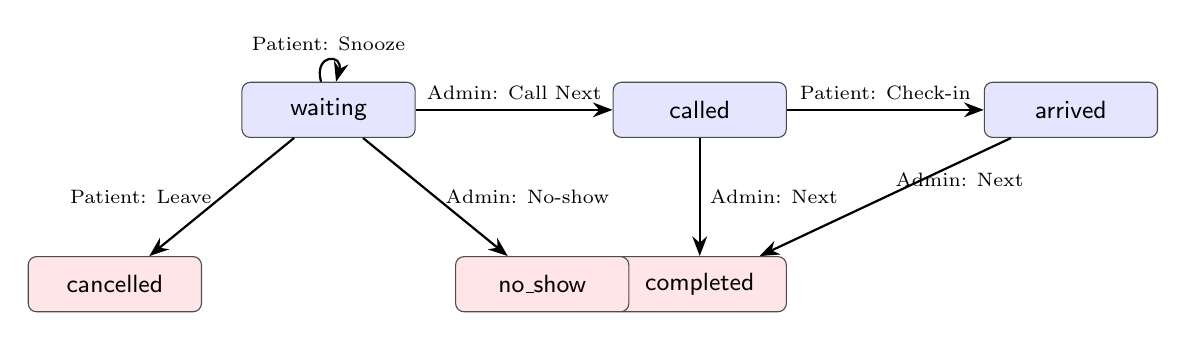
\begin{tikzpicture}[
    node distance=2cm,
    state/.style={rectangle, draw=black!70, fill=blue!10, minimum width=2.2cm, minimum height=0.7cm, font=\small\sffamily, rounded corners=3pt},
    final/.style={rectangle, draw=black!70, fill=red!10, minimum width=2.2cm, minimum height=0.7cm, font=\small\sffamily, rounded corners=3pt},
    arrow/.style={-{Stealth[length=2.5mm]}, thick}
]
    \node[state] (waiting) {waiting};
    \node[state, right=2.5cm of waiting] (called) {called};
    \node[state, right=2.5cm of called] (arrived) {arrived};
    \node[final, below=1.5cm of called] (completed) {completed};
    \node[final, below left=1.5cm and 0.5cm of waiting] (cancelled) {cancelled};
    \node[final, below right=1.5cm and 0.5cm of waiting] (noshow) {no\_show};
    
    \draw[arrow] (waiting) -- node[above, font=\scriptsize] {Admin: Call Next} (called);
    \draw[arrow] (called) -- node[above, font=\scriptsize] {Patient: Check-in} (arrived);
    \draw[arrow] (called) -- node[right, font=\scriptsize] {Admin: Next} (completed);
    \draw[arrow] (arrived) -- node[above right, font=\scriptsize] {Admin: Next} (completed);
    \draw[arrow] (waiting) -- node[left, font=\scriptsize] {Patient: Leave} (cancelled);
    \draw[arrow] (waiting) -- node[right, font=\scriptsize] {Admin: No-show} (noshow);
    
    % Self-loop for snooze
    \draw[arrow] (waiting) to[loop above, looseness=5] node[above, font=\scriptsize] {Patient: Snooze} (waiting);
\end{tikzpicture}
\caption{Token State Lifecycle Diagram}
\label{fig:token-lifecycle}
\end{figure}

% --- 4.6 High-Level Design ---
\subsection{High-Level Design (HLD)}

\subsubsection{System Architecture Diagram}

The high-level architecture of the SmartQ system follows a three-tier client-server model, as shown in Figure~\ref{fig:arch}. The client layer consists of the native Android application providing differentiated interfaces for patients, doctors, and administrators. The communication layer uses Retrofit and OkHttp for HTTP/JSON transport with JWT Bearer authentication. The API layer is an Express.js server exposing RESTful endpoints through three route modules, protected by JWT verification and role-based middleware. The data layer uses MongoDB Atlas for cloud-hosted, horizontally scalable persistence across three collections.

\begin{figure}[H]
\centering
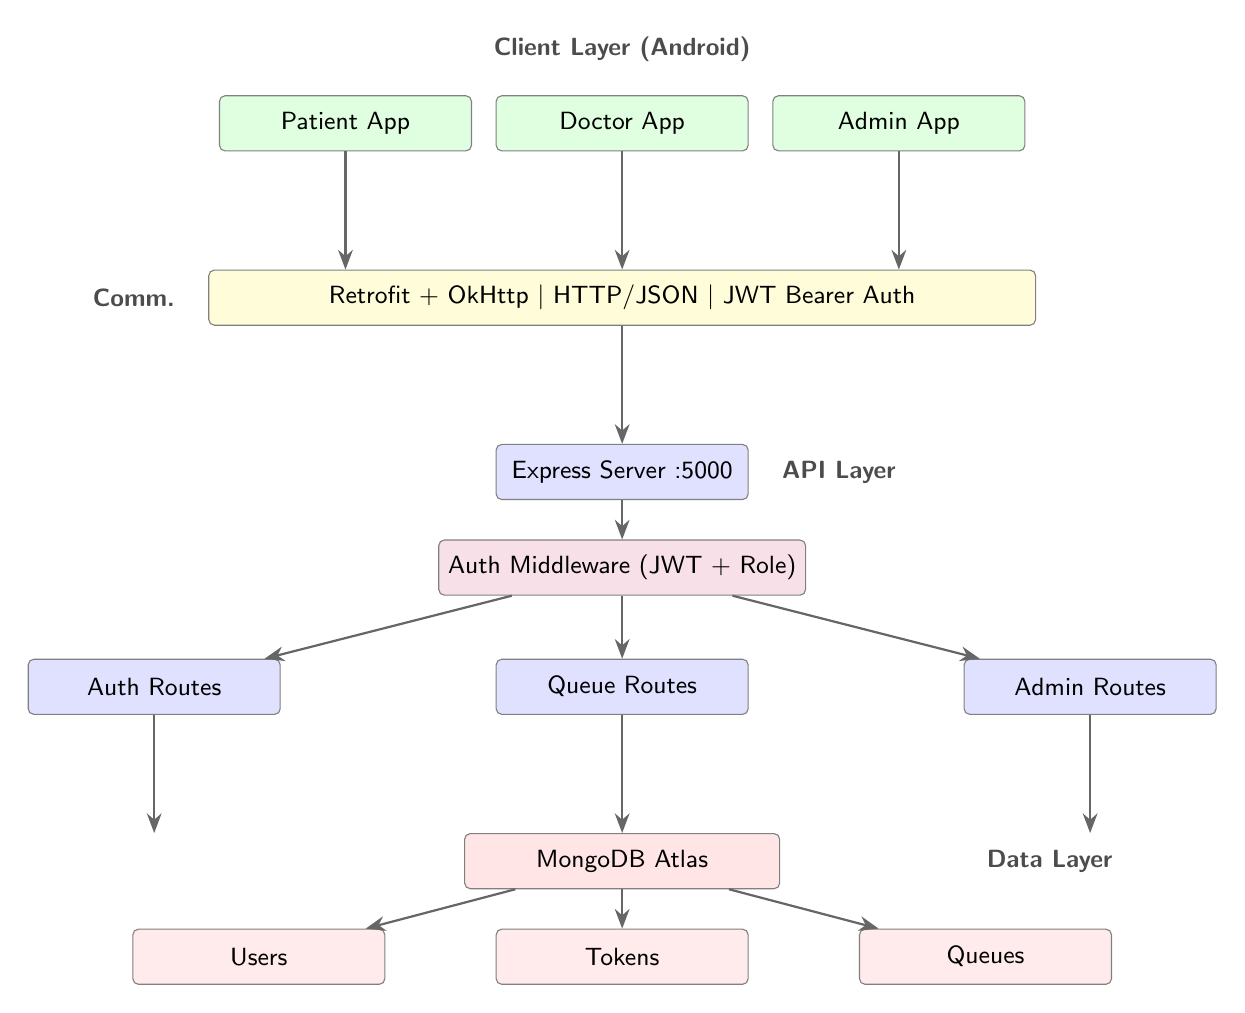
\begin{tikzpicture}[
    node distance=0.6cm,
    layer/.style={rectangle, draw=black!50, fill=#1, minimum width=3.2cm, minimum height=0.7cm, font=\small\sffamily, rounded corners=2pt},
    arrow/.style={-{Stealth[length=2.5mm]}, thick, draw=black!60},
    grouplabel/.style={font=\small\sffamily\bfseries, text=black!70}
]
    % Client Layer
    \node[layer=green!12] (patient) {Patient App};
    \node[layer=green!12, right=0.3cm of patient] (docapp) {Doctor App};
    \node[layer=green!12, right=0.3cm of docapp] (adminapp) {Admin App};
    \node[grouplabel, above=0.3cm of docapp] {Client Layer (Android)};
    
    % Communication
    \node[layer=yellow!15, below=1.5cm of docapp, minimum width=10.5cm] (comm) {Retrofit + OkHttp \textbar\ HTTP/JSON \textbar\ JWT Bearer Auth};
    \node[grouplabel, left=0.3cm of comm, anchor=east] {Comm.};
    
    % API Layer
    \node[layer=blue!12, below=1.5cm of comm] (server) {Express Server :5000};
    \node[layer=purple!12, below=0.5cm of server] (mw) {Auth Middleware (JWT + Role)};
    \node[layer=blue!12, below left=0.8cm and 2cm of mw] (authR) {Auth Routes};
    \node[layer=blue!12, below=0.8cm of mw] (queueR) {Queue Routes};
    \node[layer=blue!12, below right=0.8cm and 2cm of mw] (adminR) {Admin Routes};
    \node[grouplabel, right=0.3cm of server, anchor=west] {API Layer};
    
    % Data Layer
    \node[layer=red!10, below=1.5cm of queueR, minimum width=4cm] (mongo) {MongoDB Atlas};
    \node[layer=red!8, below left=0.5cm and 1cm of mongo] (uc) {Users};
    \node[layer=red!8, below=0.5cm of mongo] (tc) {Tokens};
    \node[layer=red!8, below right=0.5cm and 1cm of mongo] (qc) {Queues};
    \node[grouplabel, right=2.5cm of mongo, anchor=west] {Data Layer};
    
    % Arrows
    \draw[arrow] (patient.south) -- (comm.north -| patient);
    \draw[arrow] (docapp.south) -- (comm.north -| docapp);
    \draw[arrow] (adminapp.south) -- (comm.north -| adminapp);
    \draw[arrow] (comm) -- (server);
    \draw[arrow] (server) -- (mw);
    \draw[arrow] (mw) -- (authR);
    \draw[arrow] (mw) -- (queueR);
    \draw[arrow] (mw) -- (adminR);
    \draw[arrow] (authR) -- (mongo.north -| authR);
    \draw[arrow] (queueR) -- (mongo);
    \draw[arrow] (adminR) -- (mongo.north -| adminR);
    \draw[arrow] (mongo) -- (uc);
    \draw[arrow] (mongo) -- (tc);
    \draw[arrow] (mongo) -- (qc);
\end{tikzpicture}
\caption{SmartQ System Architecture Diagram}
\label{fig:arch}
\end{figure}

\subsubsection{Component Interaction Overview}

The Android application is structured using the Model-View-Controller (MVC) pattern. The \texttt{models} package contains data transfer objects (DTOs) for API requests (\texttt{LoginRequest}, \texttt{RegisterRequest}, \texttt{PrescriptionRequest}) and responses (\texttt{AuthResponse}, \texttt{QueueResponse}, \texttt{TokenResponse}, \texttt{MessageResponse}). The \texttt{network} package contains the Retrofit API interface (\texttt{ApiService}) and the singleton HTTP client (\texttt{ApiClient}). The \texttt{ui} package contains Activity classes organized by role, and the \texttt{utils} package contains the \texttt{SessionManager} for persistent session storage.

The Express.js server is organized into three route modules (\texttt{auth}, \texttt{queue}, \texttt{admin}), each handling a specific domain. Cross-cutting concerns are handled by the \texttt{authMiddleware} module, which exports \texttt{protect} (JWT verification) and \texttt{adminOnly} (role-based restriction). The MongoDB database stores all persistent data in three collections: Users (account information and priority scores), Tokens (individual queue entries per patient-doctor pair per day), and Queues (per-doctor per-day metadata including consultation time history for ETA calculation).

% --- 4.7 Low-Level Design ---
\subsection{Low-Level Design (LLD)}

\subsubsection{Database Schema Design}

The MongoDB database contains three collections: \textbf{Users}, \textbf{Tokens}, and \textbf{Queues}. The entity-relationship structure is shown in Figure~\ref{fig:er-diagram}.

\begin{figure}[H]
\centering
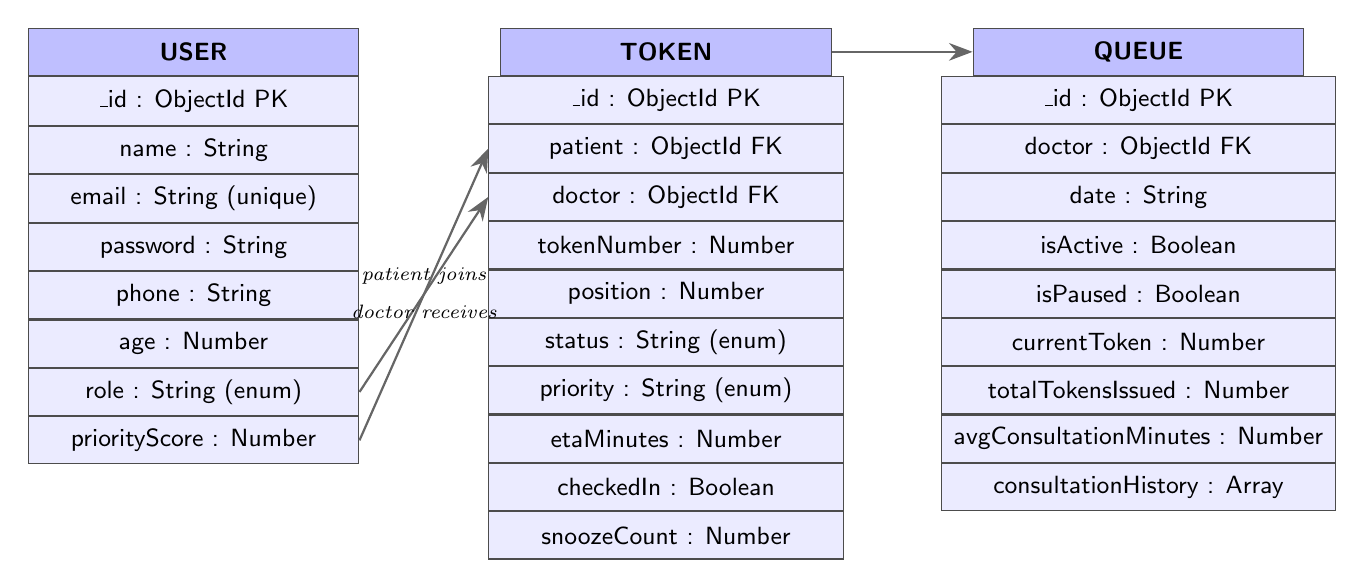
\begin{tikzpicture}[
    entity/.style={rectangle, draw=black!70, fill=blue!8, minimum width=4.2cm, minimum height=0.6cm, font=\small\sffamily},
    attr/.style={font=\footnotesize\ttfamily, text=black!80},
    title/.style={rectangle, draw=black!70, fill=blue!25, minimum width=4.2cm, minimum height=0.6cm, font=\small\sffamily\bfseries},
    rel/.style={-{Stealth[length=3mm]}, thick, draw=black!60},
]
    % USER entity
    \node[title] (ut) at (0,0) {USER};
    \node[entity, anchor=north] (u1) at (ut.south) {\begin{tabular}{l}\_id : ObjectId PK\end{tabular}};
    \node[entity, anchor=north] (u2) at (u1.south) {name : String};
    \node[entity, anchor=north] (u3) at (u2.south) {email : String (unique)};
    \node[entity, anchor=north] (u4) at (u3.south) {password : String};
    \node[entity, anchor=north] (u5) at (u4.south) {phone : String};
    \node[entity, anchor=north] (u6) at (u5.south) {age : Number};
    \node[entity, anchor=north] (u7) at (u6.south) {role : String (enum)};
    \node[entity, anchor=north] (u8) at (u7.south) {priorityScore : Number};

    % TOKEN entity
    \node[title] (tt) at (6,0) {TOKEN};
    \node[entity, anchor=north, minimum width=4.5cm] (t1) at (tt.south) {\_id : ObjectId PK};
    \node[entity, anchor=north, minimum width=4.5cm] (t2) at (t1.south) {patient : ObjectId FK};
    \node[entity, anchor=north, minimum width=4.5cm] (t3) at (t2.south) {doctor : ObjectId FK};
    \node[entity, anchor=north, minimum width=4.5cm] (t4) at (t3.south) {tokenNumber : Number};
    \node[entity, anchor=north, minimum width=4.5cm] (t5) at (t4.south) {position : Number};
    \node[entity, anchor=north, minimum width=4.5cm] (t6) at (t5.south) {status : String (enum)};
    \node[entity, anchor=north, minimum width=4.5cm] (t7) at (t6.south) {priority : String (enum)};
    \node[entity, anchor=north, minimum width=4.5cm] (t8) at (t7.south) {etaMinutes : Number};
    \node[entity, anchor=north, minimum width=4.5cm] (t9) at (t8.south) {checkedIn : Boolean};
    \node[entity, anchor=north, minimum width=4.5cm] (t10) at (t9.south) {snoozeCount : Number};

    % QUEUE entity
    \node[title] (qt) at (12,0) {QUEUE};
    \node[entity, anchor=north, minimum width=5cm] (q1) at (qt.south) {\_id : ObjectId PK};
    \node[entity, anchor=north, minimum width=5cm] (q2) at (q1.south) {doctor : ObjectId FK};
    \node[entity, anchor=north, minimum width=5cm] (q3) at (q2.south) {date : String};
    \node[entity, anchor=north, minimum width=5cm] (q4) at (q3.south) {isActive : Boolean};
    \node[entity, anchor=north, minimum width=5cm] (q5) at (q4.south) {isPaused : Boolean};
    \node[entity, anchor=north, minimum width=5cm] (q6) at (q5.south) {currentToken : Number};
    \node[entity, anchor=north, minimum width=5cm] (q7) at (q6.south) {totalTokensIssued : Number};
    \node[entity, anchor=north, minimum width=5cm] (q8) at (q7.south) {avgConsultationMinutes : Number};
    \node[entity, anchor=north, minimum width=5cm] (q9) at (q8.south) {consultationHistory : Array};

    % Relationships
    \draw[rel] (u8.east) -- node[above, font=\scriptsize\itshape] {patient joins} (t2.west);
    \draw[rel] (u7.east) -- node[below, font=\scriptsize\itshape] {doctor receives} (t3.west);
    \draw[rel] (tt.east) -- node[above, font=\scriptsize\itshape] {} (qt.west);
\end{tikzpicture}
\caption{Entity-Relationship Diagram for SmartQ Database Schema}
\label{fig:er-diagram}
\end{figure}


\subsubsection{Android Session Flow}

\begin{figure}[H]
\centering
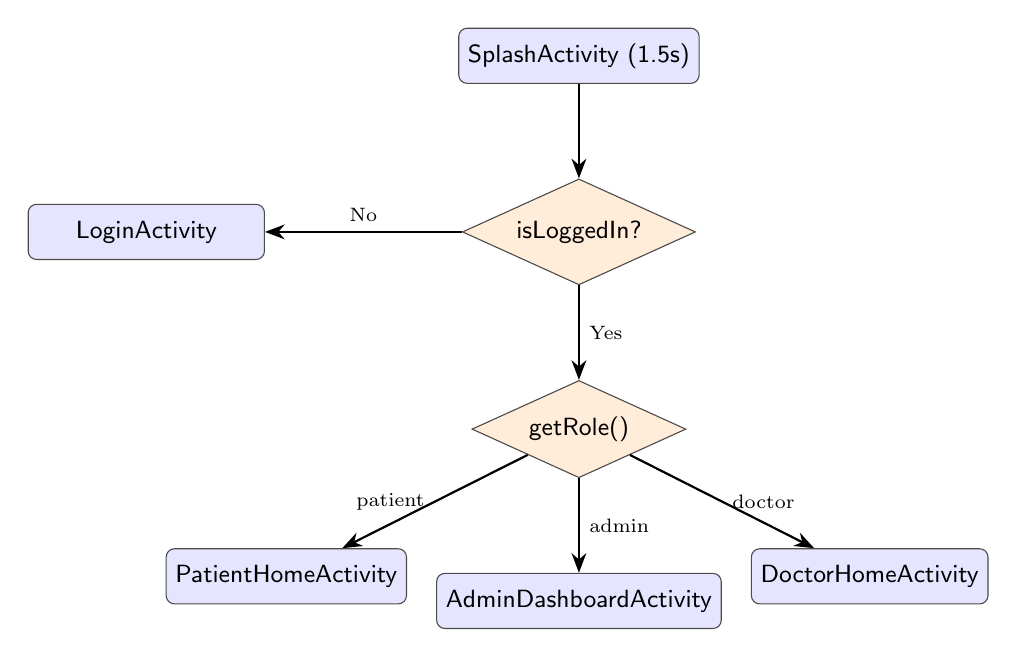
\begin{tikzpicture}[
    node distance=1.2cm,
    block/.style={rectangle, draw=black!70, fill=blue!10, minimum width=3cm, minimum height=0.7cm, font=\small\sffamily, rounded corners=3pt},
    decision/.style={diamond, draw=black!70, fill=orange!15, minimum width=1.8cm, minimum height=0.8cm, font=\small\sffamily, aspect=2.2},
    arrow/.style={-{Stealth[length=2.5mm]}, thick}
]
    \node[block] (splash) {SplashActivity (1.5s)};
    \node[decision, below=of splash] (logged) {isLoggedIn?};
    \node[block, left=2.5cm of logged] (login) {LoginActivity};
    \node[decision, below=of logged] (role) {getRole()};
    \node[block, below left=1.2cm and 1.5cm of role] (patient) {PatientHomeActivity};
    \node[block, below=of role] (admin) {AdminDashboardActivity};
    \node[block, below right=1.2cm and 1.5cm of role] (doctor) {DoctorHomeActivity};
    
    \draw[arrow] (splash) -- (logged);
    \draw[arrow] (logged) -- node[above, font=\scriptsize] {No} (login);
    \draw[arrow] (logged) -- node[right, font=\scriptsize] {Yes} (role);
    \draw[arrow] (role) -- node[left, font=\scriptsize] {patient} (patient);
    \draw[arrow] (role) -- node[right, font=\scriptsize] {admin} (admin);
    \draw[arrow] (role) -- node[right, font=\scriptsize] {doctor} (doctor);
\end{tikzpicture}
\caption{Android Session Flow Diagram}
\label{fig:session-flow}
\end{figure}

% ============================================================
% 5. CONTRIBUTION TOWARDS SOCIETY AND ENVIRONMENT
% ============================================================
\section{Contribution Towards Society and Environment}

SmartQ makes meaningful contributions to both society and the environment. By digitizing the queue management process and providing patients with real-time visibility into their wait times, the system enables patients to join queues remotely and arrive at the hospital only when their turn is approaching, thereby reducing physical overcrowding in waiting areas, lowering the risk of hospital-acquired infections, and allowing patients to utilize their waiting time productively. The automatic age-based priority triage ensures that elderly patients aged 60 and above receive preferential treatment without manual intervention, addressing a fundamental inequity in traditional first-come-first-served systems where vulnerable populations are treated identically to younger patients despite having greater medical urgency.

From an environmental perspective, SmartQ eliminates the paper waste generated by traditional token systems --- a hospital serving 500 outpatients per day produces approximately 182,500 paper tokens annually, all of which are replaced by digital tokens on the patient's smartphone. Furthermore, by reducing the need for patients to make multiple trips or wait for extended periods at the hospital, the system indirectly reduces transportation-related carbon emissions. Unlike IoT-based and kiosk-based solutions that require dedicated hardware (Raspberry Pi controllers, thermal printers, LED displays), SmartQ is entirely software-based, eliminating electronic waste associated with manufacturing and disposing of specialized equipment. The admin dashboard additionally provides hospital administrators with real-time analytics on queue lengths, consultation times, and no-show rates, enabling data-driven resource allocation and operational efficiency improvements.

% ============================================================
% 6. USE OF ADVANCED CONCEPTS
% ============================================================
\section{Use of Advanced Concepts}

The SmartQ system incorporates several advanced concepts from software engineering, data structures, algorithms, and mobile application development.

\subsection{Authentication and Security}
The system uses JSON Web Tokens (JWT) for stateless authentication, where the server creates a digitally signed token containing the user's ID and a 7-day expiration timestamp upon login. The client attaches this token as a Bearer token in the \texttt{Authorization} header of all subsequent requests, and the server verifies the signature using a secret key stored as an environment variable. Password security is ensured through bcrypt hashing with 10-round salting, guaranteeing that plain-text passwords are never stored. The backend implements a two-level middleware chain --- \texttt{protect} for JWT verification and \texttt{adminOnly} for role-based access restriction --- which are composed declaratively at the route group level using \texttt{router.use(protect, adminOnly)}.

\subsection{Algorithms and Data Consistency}
The priority triage algorithm implements a modified priority queue where patients are ordered by both priority level (high $>$ medium $>$ normal) and arrival time (FCFS within equal priority levels), using MongoDB's atomic \texttt{\$inc} operator for batch position updates to prevent race conditions during concurrent queue modifications. The ETA prediction system uses a Simple Moving Average (SMA) over the last 10 consultation durations, computed as $\text{avg} = \frac{\sum_{i=1}^{n} d_i}{n}$ where $n = \min(|\text{history}|, 10)$, ensuring adaptive estimates that converge to actual consultation pace. The Mongoose ODM's pre-save middleware hooks are used to automatically hash passwords and compute priority scores whenever a user document is modified, enforcing business rules at the data layer.

\subsection{Android Engineering Patterns}
The networking layer employs the OkHttp Interceptor design pattern to transparently attach JWT tokens to all outgoing HTTP requests, centralizing authentication logic and preventing code duplication across activities. The API contract is defined using a Java interface (\texttt{ApiService}) annotated with Retrofit annotations (\texttt{@POST}, \texttt{@GET}, \texttt{@Query}, \texttt{@Body}), which Retrofit implements at runtime via Java's dynamic proxy mechanism. Session persistence is managed through the \texttt{SessionManager} class, which uses Android's SharedPreferences API with synchronous \texttt{commit()} during logout to prevent race conditions. Real-time queue updates are achieved through a Handler-based polling mechanism in \texttt{PatientHomeActivity}, where a Runnable makes an API call and reschedules itself every 10 seconds using \texttt{postDelayed()}, with lifecycle-aware cleanup in \texttt{onDestroy()}.

% ============================================================
% 7. RESULTS AND DISCUSSIONS
% ============================================================
\section{Results and Discussions}

The SmartQ system has been successfully designed, implemented, and tested across all three phases of development.

\textbf{Authentication Module.} The registration and login flows function correctly for all three user roles. User registration validates all required fields both on the client side and server side. Duplicate email registration is properly rejected with a 409 Conflict response. Password hashing using bcrypt with 10 salt rounds ensures that plain-text passwords are never stored. JWT tokens are correctly generated and the Android client persists sessions via SharedPreferences.

\textbf{Queue Management Module.} Patients can successfully join a specific doctor's queue and receive a sequentially numbered token with an accurate initial position and ETA. The system correctly prevents duplicate token issuance. The real-time polling mechanism (10-second interval) provides reliable queue status updates, and the UI correctly transitions between three visual states: not-in-queue, in-queue, and called.

\textbf{Priority Triage Module.} The age-based priority system correctly assigns a priority score of 10 to patients aged 60+ and score 5 to others. The queue reordering algorithm correctly positions high-priority patients ahead of normal-priority patients upon joining, while preserving relative order among equal-priority patients.

\textbf{Snooze Module.} The snooze feature correctly pushes the snoozing patient back by the specified number of positions and shifts intermediate patients up. The maximum snooze limit of 2 per visit is correctly enforced.

\textbf{Check-In Module.} The manual check-in feature correctly marks the patient as physically present at the hospital. The admin dashboard correctly reflects check-in status.

\textbf{Admin Dashboard Module.} The admin dashboard correctly displays the full queue list sorted by position. The ``Call Next'' function correctly marks the current patient as completed, records the consultation duration for ETA calculation, and advances the next patient. No-show handling correctly removes patients and compacts positions.

\textbf{Dynamic ETA Accuracy.} The moving average ETA converges toward accurate predictions as consultations complete. For example, if a doctor consistently completes consultations in 5 minutes, the ETA for position~4 converges from 24 minutes $(3 \times 8)$ to 15 minutes $(3 \times 5)$ over the first 10 consultations.

\textbf{Limitations and Future Work.} The current system has several known limitations that constitute areas for future enhancement. The geofence-based automatic check-in is architecturally prepared on both the Android manifest (which declares location permissions) and the backend (which exposes the check-in endpoint), but the client-side geofence trigger using Google Play Services has not yet been implemented. Similarly, Firebase Cloud Messaging (FCM) for push notifications when a patient is called has been included as a dependency in the Android build configuration but has not yet been wired to the backend for real-time event delivery. The 10-second polling mechanism, while functional and reliable, is less efficient than WebSocket-based real-time communication and could be replaced with Socket.IO in a future iteration to reduce unnecessary network traffic and server load. From a security perspective, the JWT token expiry of 7 days is longer than recommended for healthcare applications, and implementing a refresh token mechanism with short-lived access tokens would improve the security posture. Additionally, the system currently stores JWT tokens in Android SharedPreferences, which, while convenient, is less secure than the Android Keystore system for sensitive credential storage.

% ============================================================
% 8. CONCLUSION
% ============================================================
\section{Conclusion}

The SmartQ Hospital Queue Management System has been successfully designed, developed, and tested as a comprehensive solution to the persistent problem of inefficient patient flow management in hospital outpatient departments. The system addresses six key research gaps identified in the literature survey: the absence of age-based priority triage in mobile queue systems, the lack of dynamic ETA calculation based on actual consultation durations, the missing patient-side interaction features (snooze and check-in), the absence of geofence-based arrival detection, the hardware dependency of existing solutions, and the fragmented nature of existing systems that serve only one or two user roles.

Through the implementation of a native Android application with differentiated interfaces for patients, doctors, and administrators, connected to a scalable Node.js/Express.js backend with MongoDB Atlas cloud database, SmartQ demonstrates that it is possible to build a feature-rich, secure, and cost-effective queue management solution that is entirely software-based and requires no specialized hardware. The priority triage algorithm ensures equitable care for elderly patients, the moving average ETA provides adaptive wait time predictions, and the snooze mechanism empowers patients with unprecedented control over their queue position.

The system's architecture is designed for extensibility, with provisions for geofence-based automatic check-in and FCM push notifications that can be integrated without modifying the core architecture. The use of JWT stateless authentication, bcrypt password hashing, role-based middleware chains, and atomic MongoDB operations ensures that the system is both secure and robust against concurrent access.

From a societal perspective, SmartQ contributes to reduced hospital overcrowding, elimination of paper waste from traditional token systems, reduced travel-related emissions through remote queue joining, and improved healthcare equity through automatic priority triage for elderly patients.

In conclusion, SmartQ represents a practical, deployable, and extensible contribution to the field of hospital queue management that combines mobile-first design, intelligent algorithms, and modern web technologies to deliver a significantly improved outpatient experience for patients, doctors, and hospital administrators alike.

% ============================================================
% 9. REFERENCES
% ============================================================
\section*{References}
\addcontentsline{toc}{section}{References}

\begin{enumerate}[label={[\arabic*]}]
\item A.~U.~Haq, M.~Azam, R.~Ali, and M.~Y.~Saleem, ``Mobile-Augmented Smart Queue Management System for Hospitals,'' in \textit{2020 IEEE 33rd International Symposium on Computer-Based Medical Systems (CBMS)}, IEEE, 2020, pp.~472--477. DOI:~10.1109/CBMS49503.2020.00093.

\item M.~Al-Saedi, A.~H.~M.~Alaidi, and M.~T.~Al-Khateeb, ``IoT-Based Smart Management of Healthcare Services in Hospital Buildings during COVID-19 and Future Pandemics,'' \textit{Wireless Communications and Mobile Computing}, vol.~2021, Article~ID~6680567, Hindawi, 2021. DOI:~10.1155/2021/6680567.

\item R.~Setiawan, D.~Hariyanto, and S.~Nurjanah, ``Healthcare Queue Management: IoT-Based Automated Patient Calling System for Primary Care Facilities,'' \textit{ELECTRON: Jurnal Ilmiah Teknik Elektro}, vol.~6, no.~1, 2025. DOI:~10.33795/electron.v6i1.

\item S.~Nair, A.~Menon, and R.~Krishnan, ``Smart Token Management System for Hospitals using IoT,'' \textit{Grenze International Journal of Engineering and Technology}, vol.~7, Special Issue, 2021.

\item P.~O.~Abiola, T.~S.~Oladele, and A.~A.~Adeleke, ``Predictive Queue Management in Healthcare Environments: A Systematic Review,'' \textit{World Journal of Advanced Engineering Technology and Sciences}, vol.~14, no.~2, 2025. DOI:~10.30574/wjaets.2025.14.2.

\item M.~I.~Ahmad, C.~A.~Ooi, and G.~S.~Kee, ``A Review of Patient Waiting Time Reduction Strategies in Outpatient Clinics,'' \textit{International Journal of Engineering and Advanced Technology (IJEAT)}, vol.~9, issue~1, pp.~4654--4659, 2019. ISSN:~2249-8958.

\item V.~K.~Sharma, N.~Gupta, and R.~Bhatia, ``Design and Implementation of a Queue Management System for Healthcare Using Web and Mobile Technologies,'' \textit{International Journal of Computer Science and Information Technologies (IJCSIT)}, vol.~11, no.~3, pp.~45--52, 2020. ISSN:~0975-9646.

\item D.~Konrad, K.~Meissner, and T.~Koeling, ``Analysis of Patient Flow and Waiting Times in Hospital Emergency Departments Using Discrete Event Simulation,'' \textit{Simulation Modelling Practice and Theory}, vol.~72, pp.~135--148, Elsevier, 2017. DOI:~10.1016/j.simpat.2016.12.013.

\item A.~K.~Soni, P.~Verma, and R.~S.~Chauhan, ``Securing RESTful APIs for Mobile Health Applications: A Comparative Study of Authentication Mechanisms,'' \textit{Journal of Theoretical and Applied Information Technology (JATIT)}, vol.~100, no.~4, pp.~1120--1135, 2022. ISSN:~1992-8645.

\item R.~John, S.~A.~Thomas, and P.~K.~Pillai, ``MongoDB-Based Healthcare Data Management: Performance Analysis and Scalability Evaluation,'' \textit{International Journal of Database Management Systems (IJDMS)}, vol.~13, no.~5, pp.~31--46, 2021. DOI:~10.5121/ijdms.2021.13503.
\end{enumerate}

\end{document}
